\section{Experiments}

In this section, we present the experimental setup and results of our approach. We evaluated our method only on instances of the \href{https://huggingface.co/datasets/neo4j/text2cypher-2024v1}{neo4j/text2cypher-2024v1} test set that have an already deployed Neo4j database available on the \href{https://demo.neo4jlabs.com:7473/browser/}{Demo endpoint}. This reduced the number of test instances from 4,833 to 2471, but it was strictly necessary to, at least, execute our agentic approach against the actual database used for the generation of samples in the test set. We evaluated both \textbf{effectiveness} and \textbf{efficiency} of our approach. In particular, we used already computed zero-shot and finetuned effectiveness evaluation results reported in the original paper \cite{neo4jlabs-text2cypher-2024} as several baselines to compare our approach with their one.

\subsection{Effectiveness Evaluation Metrics}

We evaluate our text-to-Cypher approach using runtime-based metrics, following the evaluation protocols established in prior work \cite{neo4jlabs-text2cypher-2024, cypherbench-megagonlabs-2024} assessing the semantic equivalence of generated Cypher queries.

\paragraph{Executable Accuracy (EA).} This metric measures whether a generated Cypher query executes successfully on the target Neo4j database without raising syntax or runtime errors. A query is considered valid if it can be executed within a specified timeout (120 seconds in our experiments) without encountering exceptions such as \texttt{CypherSyntaxError}, \texttt{DatabaseError}, \texttt{CypherTypeError}, or \texttt{ClientError}.

\paragraph{Result Similarity (RS) and Exact Match (EM).} To assess semantic equivalence at the data level, we compute the Jaccard similarity between the result sets returned by the predicted and ground truth queries. Specifically, we represent each query result as a list of dictionaries, where each dictionary corresponds to a row in the output. The similarity computation accounts for row ordering when either query contains an \texttt{ORDER BY} clause; otherwise, we apply a greedy alignment algorithm that pairs rows from both result sets to maximize overall similarity. For each aligned pair of rows, we convert values to hashable types and compute their Jaccard index. The final \textbf{Result Similarity} is the Jaccard coefficient over all (row index, value) pairs across both result sets. This metric captures whether queries retrieve the same data, even when their structural implementations differ. Following \cite{neo4jlabs-text2cypher-2024}, a value of RS $= 1$ is considered an \textbf{Exact Match}.

\paragraph{Provenance Subgraph Jaccard Similarity (PSJS).} Introduced by \cite{cypherbench-megagonlabs-2024}, this metric evaluates the structural overlap of the graph patterns matched by two queries, rather than their final result sets. The provenance subgraph of a query consists of all nodes and relationships traversed during pattern matching, regardless of what is ultimately returned. For each query, the authors \cite{cypherbench-megagonlabs-2024} extract the \texttt{MATCH} and \texttt{WHERE} clauses, augment unlabeled nodes and relationships with temporary variables, and construct a Cypher query that returns the element IDs of all matched nodes. The PSJS is then computed as the Jaccard coefficient between the sets of element IDs from the predicted and ground truth provenance subgraphs:
\[
\text{PSJS} = \frac{|PS_{\text{pred}} \cap PS_{\text{target}}|}{|PS_{\text{pred}} \cup PS_{\text{target}}|}
\]
where $PS_{\text{pred}}$ and $PS_{\text{target}}$ denote the provenance subgraphs of the predicted and target queries, respectively. This metric is particularly valuable for evaluating whether a model correctly understands the graph structure to be queried, even if the final projection or aggregation differs from the ground truth.

\paragraph{Success Rate (SR)} For each test instance, if the execution of the loop raised any exception (e.g. the graph recursion limit was reached), we assigned null values to all the evaluation metrics for that instance. In this way, we are able to clearly distinguish between failed executions and low-quality query generations. We define the Success Rate as the proportion of test instances where the agent successfully completed its execution without exceptions calling them successful sessions or instances.

\subsection{Results}

Table \ref{tab:effectiveness-results-comparison} summarizes the effectiveness of our agentic text-to-Cypher approach compared to the zero-shot and finetuned best baselines from \cite{neo4jlabs-text2cypher-2024}. As shown, our agentic approach match the best Exact Match (EM) score of $32.50\%$ achieved by the finetuned GPT-4o model, while also addressing the sub-problems \ref{itm:identify}, \ref{itm:discovery} and \ref{itm:linking} left unsolved by baselines authors \cite{neo4jlabs-text2cypher-2024}.

\begin{table}[htbp]
    \centering
    \begin{tabular}{lcccc}
        \hline
        Model & Result Similarity & Exact Match & PSJS & Success Rate \\
        \hline
        GPT-4o (zero-shot) & - & $31.73\%$ & - & - \\
        GPT-4o (fine-tuned) & - & $32.50\%$ & - & - \\
        GPT-4.1 (Ours)  & $41.22\%$ & $32.62\% $ & $69.37\%$ & $89.11\%$ \\
        % \pm 0.45 \pm 0.47 \pm 0.43
        \hline
    \end{tabular}
    \caption{Effectiveness Results Comparison with Baselines from \cite{neo4jlabs-text2cypher-2024}}
    \label{tab:effectiveness-results-comparison}
\end{table}

% \begin{table}[htbp]
%     \centering
%     \begin{tabular}{lcccc}
%         \hline
%         Model & Result Similarity & Exact Match & PSJS \\
%         \hline
%         GPT-4.1 (w/o Empty Results) & $48.50\%$ & $38.19\%$ & $82.20\%$ \\
%         GPT-4.1 (w/o NaN)  & $46.26\%$ & $36.60\%$ & $77.85\%$ \\
%         GPT-4.1 (w NaN $ = 0$)  & $41.22\%$ & $32.62\%$ & $69.37\%$ \\
%         % \pm 0.45 \pm 0.47 \pm 0.43
%         \hline
%     \end{tabular}
%     \caption{Simple example}
%     \label{tab:effectiveness-results}
% \end{table}

Figure \ref{fig:efficiency-stats} summarizes some efficiency statistics of our approach. As we can observe, from the figure \ref{fig:parallelism-distribution} that shows the distribution of the number of parallel tool calls over LLM turns, the moments in which there is the highest parallelism grade are the first 2-3 ones, where the agent exploits the available tools to quickly gather as much information as it can, hopefully reducing the overall entropy of the problem. 

The figure \ref{fig:ai-turns-distribution} shows the number of chats reaching each LLM turn, from the minimum one to the maximum one. We can observe that for the majority of the chats, the agent is able to finish its execution in less than 7-8 LLM turns, with a significant drop after the 5th-6th turn. This is coherent with the Success Rate of $89.11\%$ reported in Table \ref{tab:effectiveness-results-comparison}, which means that for the majority of the test instances, the agent is able to successfully complete its execution without exceptions.

Figures \ref{fig:no_na_df-tool-calls-distribution} and \ref{fig:df-tool-calls-distribution} (with the color legend included in table \ref{tab:tool-calls-statistics}) show the tool calls distribution over LLM turns respectively without and with the inclusion of failed chat sessions while figures \ref{fig:no_na_df-errors-distribution} and \ref{fig:df-errors-distribution} show the errors distribution over time respectively without and with the inclusion of failed chat sessions. From the first one, we can observe that, for successful sessions, the first turn is completely dominated by \textcolor{search\_for}{\rule{8pt}{4pt}}\texttt{search\_for} tool calls, which is coherent with the fact that the agent has no prior knowledge about how identified concepts are represented in the knowledge graph and it needs to perform a broad \textbf{Formalisms Discovery} to preserve recall as earliest as possible. As the turns progress, we can observe a more balanced distribution of tool calls, with \textcolor{get\_properties\_from}{\rule{8pt}{4pt}}\texttt{get\_properties\_from} and \textcolor{get\_domains\_ranges\_of}{\rule{8pt}{4pt}}\texttt{get\_domains\_ranges\_of} becoming more prominent. This indicates that as the agent gathers more information about the graph, it starts to focus on specific properties and relationships relevant to the query at hand. The appearance of \textcolor{execute\_cypher\_query}{\rule{8pt}{4pt}}\texttt{execute\_cypher\_query} tool calls, starting from the early 3rd turn, indicates that the agent has already gathered enough information to start formulating and executing Cypher queries against the database thus validating the effectiveness of the designed toolset in facilitating an efficient \textbf{Formalisms Discovery}. From the 5th turn onwards, we can observe a rapid increase in \textcolor{register\_retrieval\_result}{\rule{8pt}{4pt}}\texttt{register\_retrieval\_result} tool calls, which indicates that the agent as already solved \textbf{Concepts-Formalisms Linking} thus starting to focus on organizing and compiling the results obtained from previous tool calls to construct the final result. Combining the figure \ref{fig:no_na_df-tool-calls-distribution} and the \ref{fig:no_na_df-errors-distribution}, which shows a increasing trend of \textcolor{register\_retrieval\_result}{\rule{8pt}{4pt}}\texttt{register\_retrieval\_result} errors over LLM turns, we can infer that GPT-4.1 tend to struggle with effectively producing a valid final result due to the high complexity of the \textcolor{register\_retrieval\_result}{\rule{8pt}{4pt}}\texttt{register\_retrieval\_result} JSON Pydantic model that it must respect to successfully call the tool.

When we include failed chat sessions in the analysis (figure \ref{fig:df-tool-calls-distribution}), we can observe a similar trend until the 6th turn, after which there is a noticeable increase in \textcolor{execute\_cypher\_query}{\rule{8pt}{4pt}}\texttt{execute\_cypher\_query}, decrease in  \textcolor{register\_retrieval\_result}{\rule{8pt}{4pt}}\texttt{register\_retrieval\_result} and a more minor predominance of the \textcolor{get\_properties\_from}{\rule{8pt}{4pt}}\texttt{get\_properties\_from} tool over all the other ones. Combining this observation with the figure \ref{fig:df-errors-distribution}, which doesn't show a significant increase in \textcolor{register\_retrieval\_result}{\rule{8pt}{4pt}}\texttt{register\_retrieval\_result} errors over LLM turns, we can easily infer that for sure failed sessions were not caused by the inability of GPT-4.1 to correctly produce a valid JSON for the final result, but rather by the inherent complexity of some test instances that made the agent unable to successfully complete its execution within the imposed graph recursion limit or time constraints. This hypothesis, in fact, is further supported by the significant increase in \textcolor{execute\_cypher\_query}{\rule{8pt}{4pt}}\texttt{execute\_cypher\_query} tool calls from the 7th turn onwards without being followed by a corresponding increase in \textcolor{execute\_cypher\_query}{\rule{8pt}{4pt}}\texttt{execute\_cypher\_query} errors in figure \ref{fig:df-errors-distribution}. It can also plausibly suggest that if the agent initially took a wrong path during the \textbf{Formalisms Discovery} phase, it could be forced to execute an high number of unnecessary Cypher queries to gather more information about the graph, thus quickly reaching the graph recursion limit or time constraints without being able to recover from its initial mistake. Thus this is a strong indication that LLMs cannot effectively be used to perform probabilistic or possibilistic algorithms that require backtracking capabilities to recover from initial mistakes. All these observations suggest that \textbf{Concepts-Formalisms Linking} is still a problem that cannot easily be solved by LLMs alone in fewer than 13 turns (as the maximum number of turns observed in figure \ref{fig:ai-turns-distribution}), thus requiring further research efforts to be effectively addressed to resolve more complex text-to-Cypher tasks.

Lastly, table \ref{tab:tool-calls-statistics} shows for each tool some statistics about the number of parallel tool calls, computed in a single LLM turn, averaged over all the tool call occurrences in all the chat sessions. From the mean and standard deviation we can easily confirm the fact that GPT-4.1 was able to exploit parallelism capabilities of our designed toolset to effectively reduce the overall number of LLM turns required to complete its execution. % In particular, we can observe that the \textcolor{search\_for}{\rule{8pt}{4pt}}\texttt{search\_for} tool has the highest mean and standard deviation, which is coherent with the fact that it is the tool that is called the most in parallel during the initial \textbf{Formalisms Discovery} phase to quickly gather as much information as possible about the graph schema.

\begin{figure}[h]
  \centering
  \begin{subfigure}{0.45\textwidth}
    \centering
    \caption{N. of Parallel Tool Calls Over LLM Turns}
    \label{fig:parallelism-distribution}
    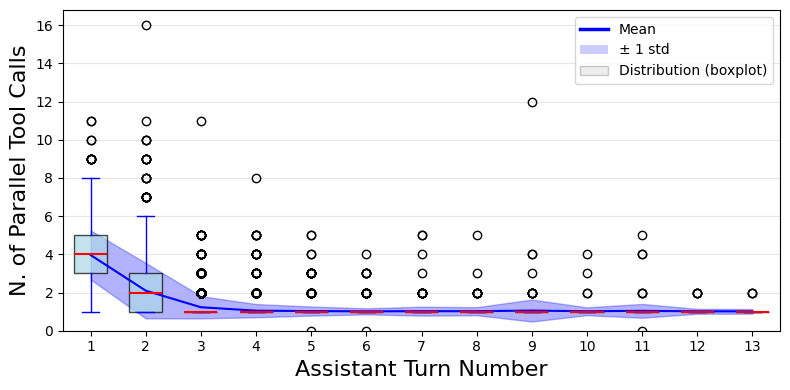
\includegraphics[width=\linewidth]{./rsc/df-parallelism-distribution-over-time.png}
  \end{subfigure}
  \hfill
  \begin{subfigure}{0.45\textwidth}
    \centering
    \caption{N. of Chats Reaching Each LLM Turn}
    \label{fig:ai-turns-distribution}
    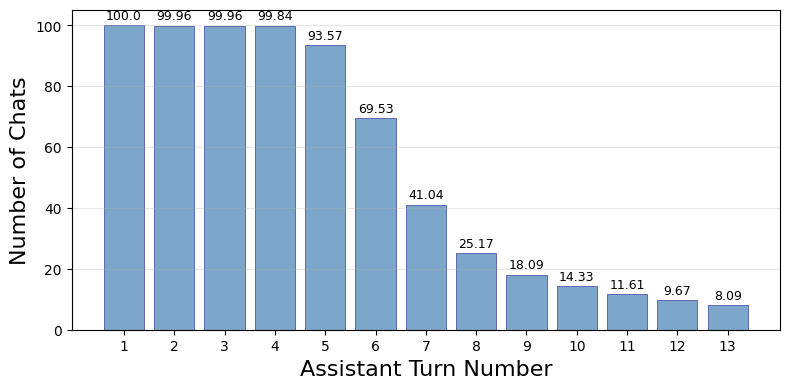
\includegraphics[width=\linewidth]{./rsc/df-ai-turns-distribution.png}
  \end{subfigure}
  \hfill
  \centering
  \begin{subfigure}{0.45\textwidth}
    \centering
    \caption{Tool Calls Distribution of only Successful Sessions Over LLM Turns}
    \label{fig:no_na_df-tool-calls-distribution}
    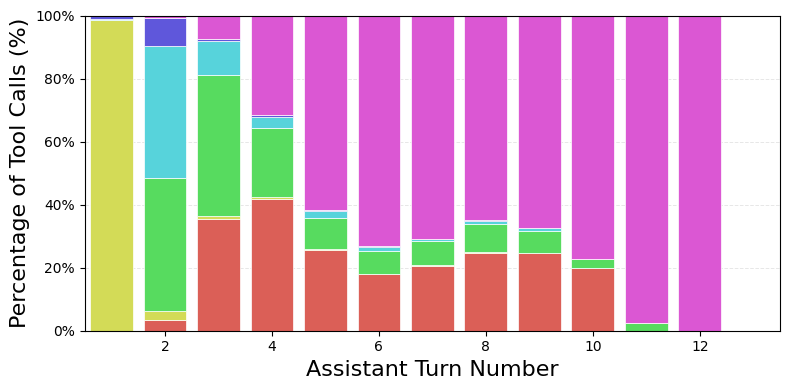
\includegraphics[width=\linewidth]{./rsc/no_na_df-tool-calls-distribution.png}
  \end{subfigure}
  \hfill
  \begin{subfigure}{0.45\textwidth}
    \centering
    \caption{Tool Calls Distribution of all Sessions Over LLMS Turns}
    \label{fig:df-tool-calls-distribution}
    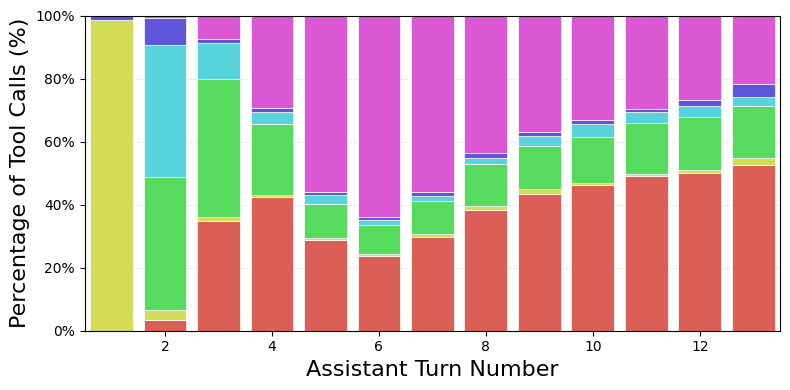
\includegraphics[width=\linewidth]{./rsc/df-tool-calls-distribution.png}
  \end{subfigure}
  \hfill
  \centering
  \begin{subfigure}{0.45\textwidth}
    \centering
    \caption{Errors Distribution of only Successful Sessions Over LLM Turns}
    \label{fig:no_na_df-errors-distribution}
    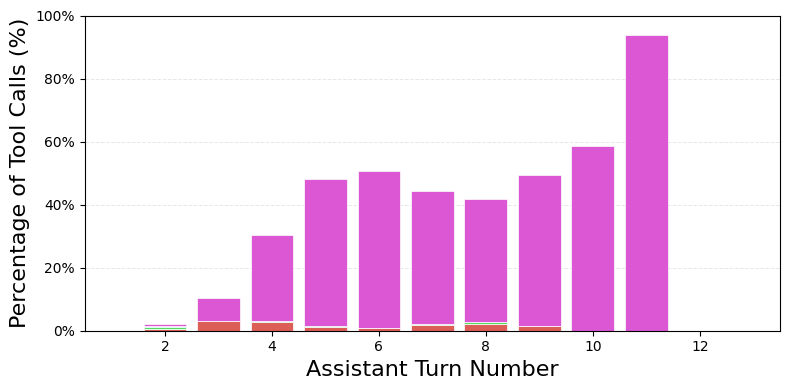
\includegraphics[width=\linewidth]{./rsc/no_na_df-errors-distribution.png}
  \end{subfigure}
  \hfill
  \begin{subfigure}{0.45\textwidth}
    \centering
    \caption{Errors Distribution of all Sessions Over LLM Turns}
    \label{fig:df-errors-distribution}
    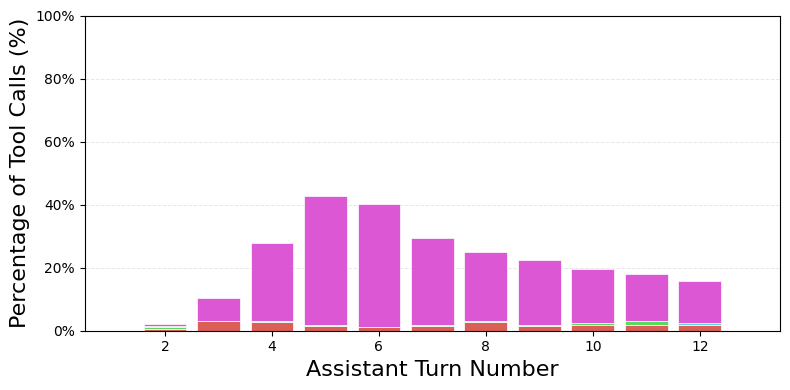
\includegraphics[width=\linewidth]{./rsc/df-errors-distribution.png}
  \end{subfigure}
  \caption{Some Efficiency Statistics}
  \label{fig:efficiency-stats}
\end{figure}

\begin{table}
    \begin{tabular}{lccccccc}
        \hline
        \textbf{Tool} & \textbf{Mean} & \textbf{Std} & \textbf{Mode} & \textbf{Min} & \textbf{Median} & \textbf{Max} & \textbf{Count} \\
        \hline
        \textcolor{execute\_cypher\_query}{\rule{8pt}{4pt}} execute\_cypher\_query                      & 1.01 & 0.10 & 1 & 1 & 1 & 4  & 4342 \\
        \textcolor{search\_for}{\rule{8pt}{4pt}} search\_for                                            & 3.69 & 1.43 & 4 & 1 & 4 & 11 & 2614 \\
        \textcolor{get\_properties\_from}{\rule{8pt}{4pt}} get\_properties\_from                        & 1.42 & 0.76 & 1 & 1 & 1 & 16 & 3813 \\
        \textcolor{get\_domains\_ranges\_of}{\rule{8pt}{4pt}} get\_domains\_ranges\_of                  & 1.46 & 0.90 & 1 & 0 & 1 & 12 & 1924 \\
        \textcolor{get\_components\_with\_property}{\rule{8pt}{4pt}} get\_components\_with\_property    & 2.05 & 1.47 & 1 & 1 & 2 & 9  & 523  \\
        \textcolor{register\_retrieval\_result}{\rule{8pt}{4pt}} register\_retrieval\_result            & 1.00 & 0.00 & 1 & 1 & 1 & 1  & 4659 \\
        \hline
    \end{tabular}
    \caption{Tool Calls Statistics}
    \label{tab:tool-calls-statistics}
\end{table}